
\subsection{Analytical solution}

As we have previously seen, Péclet's number is defined as
\begin{equation}
	\peclet = 
	\frac{\text{convection transport rate}}{\text{diffusion transport rate}} = 
	\frac{\rho v_0 L}{\Gamma}
\end{equation}
Note that the factor $\beta$ in the PDE from problem
\eqref{eq:diagonal_case_cauchy_problem} is a constant determined by the
geometry, whereas Peclet's number depends on the fluid and on the velocity
field. Since no more factors intervene on the PDE, this tells us that the
behaviour of the solution will depend greatly on Peclet's number. 

\subsubsection{Classical analytical solution for \texorpdfstring{$\mathrm{Pe} =
\infty$}{infinite Péclet's number}}

Whenever $\mathrm{Pe} \to +\infty$, it implies $\Gamma \to 0^+$ since infinite
values for the density, velocity or characteristic length make no physical
sense. Therefore the difussion coefficient tends to $0$, which means the
Laplacian term, linked to the diffusion process, is negligible. Dividing the PDE
from \eqref{eq:diagonal_case_cauchy_problem} by Péclet's number results in the
following equation
\begin{equation} \label{eq:diagonal_case_cauchy_problem_infinite_peclet_eq1}
	\pdv{\phi}{x} + \pdv{\phi}{y} = 0 \quad \text{in } \Omega
\end{equation}
The following natural step would be considering equation
\eqref{eq:diagonal_case_cauchy_problem_infinite_peclet_eq1} with $g$ as boundary
condition on all $\partial \Omega$, that is to say, the following problem:
\begin{equation} \label{eq:diagonal_case_cauchy_problem_infinite_peclet_overdetermined_problem}
	\left\{
	\begin{aligned}
		&\pdv{\phi}{x} + \pdv{\phi}{y} = 0 &
		&\text{in } \Omega \\
		&\phi = g &
		&\text{on } \partial \Omega
	\end{aligned}
	\right.
\end{equation}
Nonetheless, problem
\eqref{eq:diagonal_case_cauchy_problem_infinite_peclet_overdetermined_problem}
is ``overdetermined'', which means a part of the boundary condition is
unnecessary due to the geometric properties of the PDE as we shall see. In order
to obtain a problem we can solve, take the curve $C = \left( [0,L] \times \{ 0
\} \right) \cup \left( \{ 0 \} \times (0,L] \right)$, which is simply the lower
and left boundary, and let $\tilde{g} \colon C \subset \real^2 \rightarrow
\real$ be the function
\begin{equation}
	\tilde{g}(x,y) = 
	\left\{
	\begin{aligned}
		&\phi_\text{low} 	& &\text{if } (x,y) \in [0,L] \times \{ 0 \} \\
		&\phi_\text{high} 	& &\text{if } (x,y) \in \{ 0 \} \times (0,L] \\
	\end{aligned}
	\right.
\end{equation}
Notice that $\tilde{g}$ is the restriction of $g$ to the curve $C$, that is to
say, $\tilde{g} = g \rvert_C$. The resulting Cauchy problem is
\begin{equation} \label{eq:diagonal_case_cauchy_problem_infinite_peclet}
	\left\{
	\begin{aligned}
		&\pdv{\phi}{x} + \pdv{\phi}{y} = 0 &
		&\text{in } \Omega \\
		&\phi = g &
		&\text{on } C
	\end{aligned}
	\right.
\end{equation}
The PDE from \eqref{eq:diagonal_case_cauchy_problem_infinite_peclet} is known as the
transport equation, which is a first order linear PDE. In our case it has
constant coefficients, making it easier to solve analitically.

\begin{definition}
	A classical solution to problem
	\eqref{eq:diagonal_case_cauchy_problem_infinite_peclet} is a function $\phi
	\colon \overline{\Omega} \rightarrow \real$ that satisfies:
	\begin{enumerate}[label={(\roman*)}, topsep=0pt]
		\item $\phi \in \mathcal{C}^1(\Omega) \cap
		\mathcal{C}(\overline{\Omega})$, \ie $\phi$ is differentiable with
		continuity in $\Omega$ and continuous up to the boundary,
		\item $\phi$ satisfies the PDE, and
		\item $\phi$ satisfies the boundary conditions.
	\end{enumerate}
\end{definition}
In order to find the solution to
\eqref{eq:diagonal_case_cauchy_problem_infinite_peclet}, we will assume $\phi$
is a $\mathcal{C}^1(\Omega) \cap \mathcal{C}(\overline{\Omega})$ function. Once
we find the solution, we will be able to tell whether $\phi$ is a classical
solution, or otherwise give a meaning to $\phi$. Moreover, so as to find a
candidate of solution, we will make some assumptions motivated by intuiton and
with lack of rigour, and later we shall justify them properly. This is a common
practice in PDE theory.

We introduce some notation that will be useful. Given $m$ vectors $\vb{w}_1,
\ldots, \vb{w}_m \in \real^n$, the set $[\vb{w}_1, \ldots, \vb{w}_m] = \{
\sum_{i=1}^m \lambda_i \vb{w}_i \mid \lambda_1, \ldots, \lambda_m \in \real \}$
is the vector subspace of $\real^n$ spanned by $\vb{w}_1, \ldots, \vb{w}_m$. If
$W \subset \real^m$ is a vector subspace, $W^\perp = \{ v \in \real^n \mid v
\vdot w = 0 \ \forall w \in W \}$ is the vector subspace orthogonal to $W$.

To deduce the solution to
\eqref{eq:diagonal_case_cauchy_problem_infinite_peclet} we shall follow the
method of characteristics. Using the gradient of $\phi$ we can write the PDE as
\begin{equation} \label{eq:diagonal_case_cauchy_problem_infinite_peclet_orthogonal_vectors}
	\left( 1, 1 \right)
	\vdot
	\grad{\phi} = 
	\left( 1, 1 \right)(x,y)
	\vdot
	\begin{pmatrix}
		\displaystyle\pdv{\phi}{x} \\[10pt] \displaystyle\pdv{\phi}{y}
	\end{pmatrix} = 
	\pdv{\phi}{x}(x,y) + \pdv{\phi}{y}(x,y) = 0
\end{equation}
Recall from vector calculus that the gradient vector of $\phi$ gives the
direction of maximum growth of $\phi$ at each point, whilst a non--zero vector
$\vb{w} \in [\grad{\phi}(x,y)]^\perp$ provides the direction at $(x,y)$ along
which $\phi$ remains constant. Equation
\eqref{eq:diagonal_case_cauchy_problem_infinite_peclet_orthogonal_vectors} tells
us that at each point $(x,y) \in \Omega$, the function $\phi$ is constant along
the direction given by $(1, 1)$. To prove this claim, we may exploit the fact
that the PDE is first--order linear and use the chain rule to rewrite
\eqref{eq:diagonal_case_cauchy_problem_infinite_peclet_orthogonal_vectors}.
Consider a $\mathcal{C}^1$ mapping $\alpha(s) = (\alpha_1(s), \alpha_2(s))$ such
that $\alpha_1' = \alpha_2' = 1$ for all $s$. Since $\alpha$ is a mapping from
some subset of $\real$ to $\real^2$, its image
\begin{equation}
	A = 
	\image \alpha = 
	\left\{ (x,y) \in \real^2 \mid x = \alpha_1(s), \ y = \alpha_2(s), \ s \in \real \right\}
\end{equation}
can be thought of as a $\mathcal{C}^1$. Moreover, we may choose the curve to
pass through $\Omega \cup C$ as we shall see in a moment. The restriction of $\phi$
to $A$, given by the composition $\varphi = \phi \circ \alpha \colon I \subset
\real \rightarrow \real$, is also a $\mathcal{C}^1$ function as it is
composition of $\mathcal{C}^1$ functions. By the chain rule,
\begin{equation} \label{eq:diagonal_case_cauchy_problem_infinite_peclet_chain_rule}
	\frac{\dd}{\dd{s}} \varphi(s) = 
	\frac{\dd}{\dd{s}} \phi(\alpha_1(s), \alpha_2(s)) = 
	\frac{\partial \phi}{\partial x} (\alpha_1(s), \alpha_2(s)) \alpha_1'(s) +  	
	\frac{\partial \phi}{\partial y} (\alpha_1(s), \alpha_2(s)) \alpha_2'(s) =
	\pdv{\phi}{x} + \pdv{\phi}{y} = 0
\end{equation}
where the last equality holds whenever $\alpha(s) \in \Omega$. Equation
\eqref{eq:diagonal_case_cauchy_problem_infinite_peclet_chain_rule} implies that
$\phi$ is constant on every connected component of $A \cap
\Omega$, thereby proving our claim. 

The following step is to find the curve $A$. Consider the mapping 
\begin{equation}
	\begin{aligned}
		f \colon \real^3 &\longrightarrow \real^2 \\
		(s,x,y) &\longmapsto f(s,x,y) = (1,1)
	\end{aligned}
\end{equation}
By taking a point $(x_0, y_0) \in \Omega \cup C$ contained in $A$, the following Cauchy
problem arises naturally:
\begin{equation} \label{eq:diagonal_case_cauchy_problem_infinite_peclet_characteristics_problem}
	\left\{
		\begin{aligned}
			&\alpha'(s) = 
			(\alpha_1'(s), \alpha_2'(s)) = 
			f(s,\alpha_1(s),\alpha_2(s)) =
			(1,1) & &\text{in } I \subset \real \\
			&\alpha(0) = 
			(\alpha_1(0), \alpha_2(0)) = 
			(x_0, y_0)
		\end{aligned}
	\right.
\end{equation}
The function $f$ is constant, therefore is Lipschitz continuous on $(x,y)$ and
uniformly with respect to $s$, hence the solution to
\eqref{eq:diagonal_case_cauchy_problem_infinite_peclet_characteristics_problem}
exists and is unique due to the Picard--Lindelöf Theorem (Theorem
\ref{teo:picard_lindelof}). In addition, it is given by
\begin{equation} \label{eq:diagonal_case_cauchy_problem_infinite_peclet_characteristics_solution}
	\alpha(s) = (x_0 + s, y_0 + s) = (x_0, y_0) + s(1, 1) \quad s \in I \subset \real
\end{equation}
whence $A$ is the line passing by $(x_0, y_0)$ with director subspace $[(1,
1)]$. Moreover $A$ is not a single line, but rather a family of lines with
different initial condition. Hereinafter, we take the initial condition to be in
the lower or left boundary, that is to say, $(x_0,y_0) \in C$\footnote{We take
$(x_0,y_0) \in C$ because at those points we have the boundary condition, \ie we
have information about the solution $\phi$.}. To distinguish the solutions
\eqref{eq:diagonal_case_cauchy_problem_infinite_peclet_characteristics_problem}
we will denote them by $\alpha(s; x_0, y_0)$, and the curves by $A_{(x_0,y_0)}$.

\begin{figure}[ht]
	\centering
	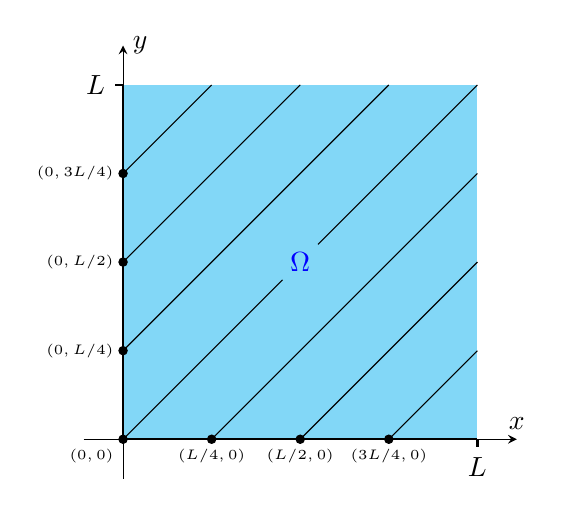
\begin{tikzpicture}
		% Lenghts
		\def\alength{5}
		\def\L{4.5}
		\def\mlength{0.1}
		% Axis
		\draw[-stealth] (0,-0.5) -- (0,\alength) node[right]{$y$};
		\draw[-stealth] (-0.5,0) -- (\alength,0) node[above]{$x$};
		\draw[black, thick] (\L,0) -- ++(0,-\mlength) node[below]{$L$};
		\draw[black, thick] (0,\L) -- ++(-\mlength,0) node[left]{$L$};
		% Domain
		\fill[cyan!70!white,opacity=0.7] (0,0) rectangle (\L, \L);
		\draw[thick, thick] (0,\L) -- (0,0) -- (\L,0);
		% Characteristics
%		\draw[black] (0,0) -- node[midway, above, rotate=45]{\tiny{$x - y = 0$}} (\L, \L);
		\node[blue] at ({0.5*\L}, {0.5*\L}) {$\Omega$};
		\draw[black] (0,0) -- ({0.45*\L}, {0.45*\L});
		\draw[black] ({0.55*\L}, {0.55*\L}) -- (\L, \L);		
		\draw[black] ({0.25*\L}, 0) -- (\L, {0.75*\L});
		\draw[black] ({0.50*\L}, 0) -- (\L, {0.50*\L});
		\draw[black] ({0.75*\L}, 0) -- (\L, {0.25*\L});		
		\draw[black] (0, {0.25*\L}) -- ({0.75*\L}, \L);
		\draw[black] (0, {0.50*\L}) -- ({0.50*\L}, \L);
		\draw[black] (0, {0.75*\L}) -- ({0.25*\L}, \L);
		% Points
		\filldraw[black] (0,{0.75*\L}) circle (1.5pt);
		\filldraw[black] (0,{0.50*\L}) circle (1.5pt);
		\filldraw[black] (0,{0.25*\L}) circle (1.5pt);
		\filldraw[black] (0,0) circle (1.5pt);
		\filldraw[black] ({0.25*\L},0) circle (1.5pt);
		\filldraw[black] ({0.50*\L},0) circle (1.5pt);
		\filldraw[black] ({0.75*\L},0) circle (1.5pt);
		% Text
		\node[black, anchor=east] at (0,{0.75*\L}) {\tiny{$(0,3L/4)$}};
		\node[black, anchor=east] at (0,{0.50*\L}) {\tiny{$(0,L/2)$}};
		\node[black, anchor=east] at (0,{0.25*\L}) {\tiny{$(0,L/4)$}};
		\node[black, anchor=north east] at (0,0) {\tiny{$(0,0)$}};
		\node[black, anchor=north] at ({0.25*\L},0) {\tiny{$(L/4,0)$}};
		\node[black, anchor=north] at ({0.50*\L},0) {\tiny{$(L/2,0)$}};
		\node[black, anchor=north] at ({0.75*\L},0) {\tiny{$(3L/4,0)$}};
	\end{tikzpicture}
	\captionsetup{width=0.70\linewidth}
	\caption{Some of the lines given by
	\eqref{eq:diagonal_case_cauchy_problem_infinite_peclet_characteristics_solution}
	with initial condition $(x_0,y_0) \in C$ extended to the top and right
	boundaries of $\Omega$.}
	\label{fig:diagonal_case_cauchy_problem_infinite_peclet_lines_from_C}
\end{figure}

We claim that a solution
\eqref{eq:diagonal_case_cauchy_problem_infinite_peclet_characteristics_solution}
can be extended so that $\alpha(s;x_0,y_0)$ eventually reaches the top or right
boundaries of $\Omega$ as shown in figure
\ref{fig:diagonal_case_cauchy_problem_infinite_peclet_lines_from_C}. Take $T >
0$ and $\delta > 0$ to be some constants to be determined and let $V = [0, T]
\times \overline{B((x_0,y_0), \delta)} \subset \real^3$. Since $f$ is a constant
function, we have
\begin{equation}
	M = 
	\sup_{(s,x,y) \in V} \norm{f(s,x,y)} = 
	\max_{(s,x,y) \in V} \norm{f(s,x,y)} = 
	\sqrt{2}
\end{equation} 
Again, by the Picard--Lindelöf theorem, the solution
\eqref{eq:diagonal_case_cauchy_problem_infinite_peclet_characteristics_solution}
exists for $s \in I = [0, T_0] \subset \real$ and remains in
$\overline{B((x_0,y_0), \delta)}$ where $T_0 = \min{\left\{ T, \frac{\delta}{M}
\right\}}$. By taking $\delta = \sqrt{2} L$ and $T = L$, applying the theorem we
obtain $T_0 = L$ and the solution stays in $\overline{B((x_0,y_0), \sqrt{2}
L)}$. Since $\sqrt{2} L$ is the maximum of the distances between two points
belonging to $\overline{\Omega}$, we have proved our claim. As a consequence, by
changing $(x_0,y_0)$ we can fill $\overline{\Omega}$ with these curves. All
except one of the solutions $\alpha(s;x_0,y_0)$ actually exit
$\overline{\Omega}$, however we do not care about the part of the curve outside
$\overline{\Omega}$\footnote{We have such freedom to choose the constants $T$
and $\delta$ because $f$ is a constant function.}.

Up to now, we have found out the following:
\begin{enumerate}[label={(\roman*)}, topsep=0pt]
	\item The lines given by $\alpha(s;x_0,y_0)$ can extended so that both ends
	touch $\partial \Omega$. The implicit form of these is
	\begin{equation} \label{eq:diagonal_case_cauchy_problem_infinite_peclet_characteristics_implicit_form}
		A_{(x_0,y_0)} \colon x - y = x_0 - y_0, \quad (x_0,y_0) \in C
	\end{equation}
	\item The lines
	\eqref{eq:diagonal_case_cauchy_problem_infinite_peclet_characteristics_implicit_form}
	fill $\overline{\Omega}$.
	\item By equation
	\eqref{eq:diagonal_case_cauchy_problem_infinite_peclet_chain_rule}, the
	function $\phi$ is constant on every line
	\eqref{eq:diagonal_case_cauchy_problem_infinite_peclet_characteristics_implicit_form}.
	\label{eq:infinite_peclet_point_2}
\end{enumerate}
The curves
\eqref{eq:diagonal_case_cauchy_problem_infinite_peclet_characteristics_implicit_form}
are known as the characteristic lines (or simply characteristics) of problem
\eqref{eq:diagonal_case_cauchy_problem_infinite_peclet}. Some of them are
picture in figure
\ref{fig:diagonal_case_cauchy_problem_infinite_peclet_characteristics_problem}.

\begin{figure}[ht]
	\centering
	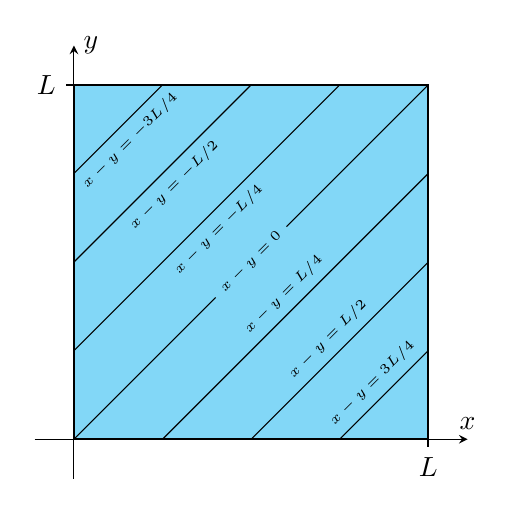
\begin{tikzpicture}
		% Lenghts
		\def\alength{5}
		\def\L{4.5}
		\def\mlength{0.1}
		% Axis
		\draw[-stealth] (0,-0.5) -- (0,\alength) node[right]{$y$};
		\draw[-stealth] (-0.5,0) -- (\alength,0) node[above]{$x$};
		\draw[black, thick] (\L,0) -- ++(0,-\mlength) node[below]{$L$};
		\draw[black, thick] (0,\L) -- ++(-\mlength,0) node[left]{$L$};
		% Domain
		\fill[cyan!70!white,opacity=0.7] (0,0) rectangle (\L, \L);
		\draw[thick, thick] (0,0) rectangle (\L, \L);
		% Characteristics
%		\draw[black] (0,0) -- node[midway, above, rotate=45]{\tiny{$x - y = 0$}} (\L, \L);
		\node[rotate=45] at ({0.5*\L}, {0.5*\L}) {\tiny{$x - y = 0$}};
		\draw[black] (0,0) -- ({0.4*\L}, {0.4*\L});
		\draw[black] ({0.6*\L}, {0.6*\L}) -- (\L, \L);
		
		\draw[black] ({0.25*\L}, 0) -- node[midway, above, rotate=45]{\tiny{$x - y = L/4$}} 
		(\L, {0.75*\L});
		\draw[black] ({0.50*\L}, 0) -- node[midway, above, rotate=45]{\tiny{$x - y = L/2$}} 
		(\L, {0.50*\L});
		\draw[black] ({0.75*\L}, 0) -- node[midway, above, rotate=45]{\tiny{$x - y = 3L/4$}} 
		(\L, {0.25*\L});
		
		
		
		\draw[black] (0, {0.25*\L}) -- node[midway, below, rotate=45]{\tiny{$x - y = -L/4$}} 
		({0.75*\L}, \L);
		\draw[black] (0, {0.50*\L}) -- node[midway, below, rotate=45]{\tiny{$x - y = -L/2$}} 
		({0.50*\L}, \L);
		\draw[black] (0, {0.75*\L}) -- node[midway, below, rotate=45]{\tiny{$x - y = -3L/4$}} 
		({0.25*\L}, \L);
	\end{tikzpicture}
	\caption{Some characteristics of problem \eqref{eq:diagonal_case_cauchy_problem_infinite_peclet}.}
	\label{fig:diagonal_case_cauchy_problem_infinite_peclet_characteristics_problem}
\end{figure}

We know the value of $\phi$ at $(x_0,y_0) \in C$ and $\phi$ is constant along
the curve $A_{(x_0,y_0)}$. Therefore the value of $\phi$ at $(x,y) \in
A_{(x_0,y_0)}$ is $\phi(x,y) = \phi(x_0,y_0) = \tilde{g}(x_0,y_0)$. As
$(x_0,y_0) \in C$ implies either $x_0 = 0$ or $y_0 = 0$ (or both), we have the following:
\begin{itemize}[topsep=0pt]
	\item If $y \leq x$ then $\phi(x,y) = \phi(x-y,0) = \tilde{g}(x-y,0)$.
	\item If $y > x$ then $\phi(x,y) = \phi(0,y-x) = \tilde{g}(0,y-x)$.
\end{itemize}
With this in mind, the solution to \eqref{eq:diagonal_case_cauchy_problem_infinite_peclet} is:
\begin{equation} \label{eq:diag_inf_pe_solution}
	\phi(x,y) = 
	\left\{
		\begin{aligned}
			&\tilde{g}(x-y,0) = \phi_\text{low} & &\text{if } y \leq x \\
			&\tilde{g}(0,y-x) = \phi_\text{high} & &\text{if } y > x \\
		\end{aligned}
	\right.
	\quad
	(x,y) \in \overline{\Omega}
\end{equation}
Intuitively, the characteristics give the paths in $\real^2$ through which the
information of the boundary conditions is transported. 

After finding the solution, we should check if $\phi \in \mathcal{C}^1(\Omega)
\cap \mathcal{C}(\overline{\Omega})$. First consider the case when
$\phi_\text{low} = \phi_\text{high}$.

\begin{theorem}
	Assume $\phi_\text{low} = \phi_\text{high}$. Then the solution to problem
	\eqref{eq:diagonal_case_cauchy_problem_infinite_peclet} exists, is unique
	and is a solution in the classical sense.
\end{theorem}
\begin{proof}
	We have proved the existence of a solution by giving the formula
	\eqref{eq:diag_inf_pe_solution}. The uniqueness is a consequence of the
	method of characteristics. In it we have seen that $\phi$ is constant on
	each the characteristic, then we have found the equation of characteristics
	and and proved that given an initial condition $(x_0,y_0) \in C$, the curve
	is unique. Finally $\phi$ is a $\mathcal{C}^1(\Omega) \cap
	\mathcal{C}(\overline{\Omega})$ function because it is constant on
	$\overline{\Omega}$ and clearly satisfies the boundary condition by
	construction and the PDE.
\end{proof}

Assume that $\phi_\text{low} < \phi_\text{high}$. Then $\phi$ is not continuous
on the segment $\{ x - y = 0 \} \cap \overline{\Omega}$ thus it cannot be a
differentiable function. Therefore function \eqref{eq:diag_inf_pe_solution} is
not a classical solution. Furthermore it could be warned from the beginning that
problem \eqref{eq:diagonal_case_cauchy_problem_infinite_peclet} does not admit
classical solution as any function satisfying the boundary condition is not
continuous at $(0,0)$.


\subsubsection{Weak analytical solution for \texorpdfstring{$\mathrm{Pe} =
\infty$}{infinite Péclet's number}}


As we have seen in the previous subsection, problem 

\begin{definition}
	A function $\psi \colon \overline{\Omega} \rightarrow \real$ is said to be a
	weak solution of problem
	\eqref{eq:diagonal_case_cauchy_problem_infinite_peclet} if for all test
	functions $\psi \in \mathcal{C}^1_c (\overline{\Omega})$ the following
	integral equation is satisfied:
	\begin{equation}
		\int_\Omega 
	\end{equation}
	
	A function $\psi \colon \overline{\Omega} \rightarrow \real$
	is said a weak solution of
	\eqref{eq:diagonal_case_cauchy_problem_infinite_peclet} if 
	\[
		\int_\Omega 
	\]
\end{definition}


Notice that each characteristic starting on $C_1$ ends on $C_1$, and the same
holds for $C_2$. 

y definition of the Cauchy problem, $\phi$ is
constant on $C_1$ and on $C_2$. Therefore the value of $\phi$ on the
characteristic $x - y = c$ is the value that $g$ takes on the part of the
boundary the characteristic intersects.
% \subsubsection{Analytical solution for \texorpdfstring{$\peclet = 0$}{zero Péclet's number}}

Now we consider the problem \eqref{eq:diagonal_case_cauchy_problem} when $\peclet \to 0$. Since $\rho > 0$ and $L > 0$, the fact that Péclet's number is close to zero implies that velocity $u$ is close to zero. In the extreme case when $u = 0$, there is no transport, therefore $\peclet = 0$ and problem \eqref{eq:diagonal_case_cauchy_problem} becomes
\begin{equation} \label{eq:diagonal_case_cauchy_problem_zero_peclet}
	\left\{
	\begin{aligned}
		&\Delta \phi = 0 &
		&\text{in } \Omega \\
		&\phi = g &
		&\text{on } \partial \Omega
	\end{aligned}
	\right.
\end{equation}
which is Laplace's problem in the square $\Omega$. 
\subsubsection{General problem}

Hereinafter we consider problem \eqref{eq:diagonal_case_cauchy_problem} with $0
< \peclet < +\infty$ with $\phi_\text{low} < \phi_\text{high}$. To begin, we
focus on the existence of classical solution.

\begin{definition}
	A classical solution to problem
	\eqref{eq:diagonal_case_cauchy_problem_infinite_peclet} is a function $\phi
	\colon \overline{\Omega} \rightarrow \real$ that satisfies:
	\begin{enumerate}[label={(\roman*)}, topsep=0pt]
		\item $\phi \in \mathcal{C}^2(\Omega) \cap
		\mathcal{C}(\overline{\Omega})$,
		\item $\phi$ satisfies the PDE, and
		\item $\phi$ satisfies the boundary conditions.
	\end{enumerate}
\end{definition}

\noindent
The function $g$ giving the boundary conditions is not continuous at $(0,0)$ nor
at $(L, L)$ unless $\phi_\text{low} = \phi_\text{high}$. Therefore problem
\eqref{eq:diagonal_case_cauchy_problem} cannot have a classical solution.
Nonetheless it might have a solution in the weak sense.

Before studying the theorem that deals with the existence of a weak 

\begin{definition}
	contenidos...
\end{definition}

\subsubsection{Expected nature of the solution}

